% Don't touch this %%%%%%%%%%%%%%%%%%%%%%%%%%%%%%%%%%%%%%%%%%%
\documentclass[12pt]{article}
\usepackage{fullpage}
\usepackage[left=1in,top=1in,right=1in,bottom=1in,headheight=3ex,headsep=3ex]{geometry}
\usepackage{graphicx}
\usepackage{float}
\usepackage{array}


\newcommand{\blankline}{\quad\pagebreak[2]}
%%%%%%%%%%%%%%%%%%%%%%%%%%%%%%%%%%%%%%%%%%%%%%%%%%%%%%%%%%%%%%

% Modify Course title, instructor name, semester here %%%%%%%%

\title{Homework 3: Oscillations and waves}
\author{PHY250 - Fall 2021}
\date{}

%%%%%%%%%%%%%%%%%%%%%%%%%%%%%%%%%%%%%%%%%%%%%%%%%%%%%%%%%%%%%%

% Don't touch this %%%%%%%%%%%%%%%%%%%%%%%%%%%%%%%%%%%%%%%%%%%
\usepackage[sc]{mathpazo}
%\linespread{1.05} % Palatino needs more leading (space between lines)
\usepackage[T1]{fontenc}
\usepackage[mmddyyyy]{datetime}% http://ctan.org/pkg/datetime
\usepackage{advdate}% http://ctan.org/pkg/advdate

\usepackage{setspace}

\newcommand{\HRule}{\rule{\linewidth}{0.5mm}}
\newdateformat{syldate}{\twodigit{\THEMONTH}/\twodigit{\THEDAY}}
\newsavebox{\MONDAY}\savebox{\MONDAY}{Mon}% Mon
\newcommand{\week}[1]{%
%  \cleardate{mydate}% Clear date
% \newdate{mydate}{\the\day}{\the\month}{\the\year}% Store date
  \paragraph*{\kern-2ex\quad #1, \syldate{\today} - \AdvanceDate[4]\syldate{\today}:}% Set heading  \quad #1
%  \setbox1=\hbox{\shortdayofweekname{\getdateday{mydate}}{\getdatemonth{mydate}}{\getdateyear{mydate}}}%
  \ifdim\wd1=\wd\MONDAY
    \AdvanceDate[7]
  \else
    \AdvanceDate[7]
  \fi%
}
%\usepackage{setspace}
\usepackage{multicol}
%\usepackage{indentfirst}
\usepackage{fancyhdr,lastpage}
\usepackage{url}
\pagestyle{fancy}
\usepackage{hyperref}
\usepackage{lastpage}
\usepackage{amsmath}
\usepackage{layout}

\lhead{}
\chead{}
%%%%%%%%%%%%%%%%%%%%%%%%%%%%%%%%%%%%%%%%%%%%%%%%%%%%%%%%%%%%%%

% Modify header here %%%%%%%%%%%%%%%%%%%%%%%%%%%%%%%%%%%%%%%%%
%\rhead{\footnotesize Text in header}

%%%%%%%%%%%%%%%%%%%%%%%%%%%%%%%%%%%%%%%%%%%%%%%%%%%%%%%%%%%%%%
% Don't touch this %%%%%%%%%%%%%%%%%%%%%%%%%%%%%%%%%%%%%%%%%%%
\lfoot{}
\cfoot{\small \thepage/\pageref*{LastPage}}
\rfoot{}

\usepackage{array, xcolor}
\usepackage{color,hyperref}
\definecolor{clemsonorange}{HTML}{EA6A20}
\hypersetup{colorlinks,breaklinks,linkcolor=clemsonorange,urlcolor=clemsonorange,anchorcolor=clemsonorange,citecolor=black}



\begin{document}


\maketitle

\textcolor{red}{Deadline: 10/25/2021}

\vspace{5mm}

\begin{spacing}{0.3}
    \noindent
    \HRule\\
    \HRule
\end{spacing}
\vspace{5mm}


% First Section %%%%%%%%%%%%%%%%%%%%%%%%%%%%%%%%%%%%%%%%%%%%


\newcounter{example}
\setcounter{example}{1}

\section*{Exercise \theexample \footnote{14.57 from Sears and Zemansky}}
The two pendulums shown in Fig. \ref{1}  each consist
of a uniform solid ball of mass M supported by a rigid massless
rod, but the ball for pendulum A is very tiny while the ball for pendulum
B is much larger. Find the period of each pendulum for
small displacements. Which ball takes longer to complete a swing?

\begin{figure}[h!]
  \begin{center}
    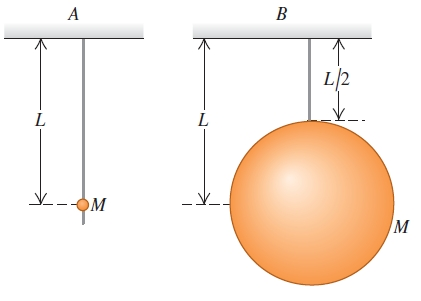
\includegraphics[height=2.in]{images/1.jpg}
    \caption{Exercise \theexample }
    \label{1}
  \end{center}
\end{figure}


% Second Section %%%%%%%%%%%%%%%%%%%%%%%%%%%%%%%%%%%%%%%%%%%%

\stepcounter{example}

\section*{Exercise \theexample \footnote{14.76  from Sears and Zemansky}}

An object with
height h, mass M, and a uniform cross-sectional area A floats
upright in a liquid with density $\rho$ (a) Calculate the vertical distance
from the surface of the liquid to the bottom of the floating
object at equilibrium. (b) A downward force with magnitude F is
applied to the top of the object. At the new equilibrium position,
how much farther below the surface of the liquid is the bottom of
the object than it was in part (a)? (Assume that some of the object
remains above the surface of the liquid.) (c) Your result in part (b)
shows that if the force is suddenly removed, the object will oscillate
up and down in SHM. Calculate the period of this motion in
terms of the density $\rho$ of the liquid, the mass M, and the crosssectional
area A of the object. You can ignore the damping due to
fluid friction.




\stepcounter{example}

\section*{Exercise \theexample \footnote{15.21 from Sears and Zemansky}}


A simple harmonic oscillator at the point $x=0$ generates
a wave on a rope. The oscillator operates at a frequency of 40.0 Hz
and with an amplitude of $3.00 cm$. The rope has a linear mass density
of $50~g/m$ and is stretched with a tension of 5.00 N.
(a) Determine the speed of the wave. (b) Find the wavelength.
(c) Write the wave function $y(x,t)$ for the wave. Assume that the
oscillator has its maximum upward displacement at time $t=0$
(d) Find the maximum transverse acceleration of points on the
rope. (e) In the discussion of transverse waves  the
force of gravity was ignored. Is that a reasonable approximation
for this wave? Explain.



\stepcounter{example}

\section*{Exercise \theexample \footnote{15.75 from Sears and Zemansky}}

A string that lies along the $+x$-axis has a free end
at $x=0$. (a) Show that an incident traveling wave $y_1(x,t)=Acos(kx+\omega )$ 
gives rise to a standing wave $y(x,t)=2Acos(\omega )cos(k x)$ 
(b) Show that the standing wave has an antinode
at its free end (x=0) (c) Find the maximum displacement, maximum
speed, and maximum acceleration of the free end of the string. (d) find the resonance frequencies 
for the system.


\end{document}


